\documentclass{article}

% Maths
\usepackage{amsmath}

% Hyperlink
\usepackage{hyperref}
\hypersetup{
    colorlinks=true,
    linkcolor=blue,
    filecolor=magenta,      
    urlcolor=cyan,
    pdfpagemode=FullScreen,
}

% Figures
\usepackage{graphics, float, subfig}
\usepackage[pdflatex]{graphicx}

% Itemize
\renewcommand{\labelitemi}{\textbullet}
\renewcommand{\labelitemii}{\textbullet}
\renewcommand{\labelitemiii}{\textbullet}

% Margins
\usepackage[margin=1in]{geometry}

% Helpful commands
\newcommand{\x}{\mathbf{x}}
\newcommand{\A}{\mathbf{A}}
\newcommand{\B}{\mathbf{b}} % \b already defined
\newcommand{\I}{\mathbf{I}}

\begin{document}

% TODO: Make a nice title page
APPM 4600 Project 3: Regularization in Least Squares\\
Alexey Yermakov, Logan Barnhart, and Tyler Jensen

\section{Ridge Regression}
\subsection{Deriving the Ridge Estimator}

The equation for regularized least squares is:

\begin{equation} \label{eqn:rls}
    \arg \min_{x} ||\A\x-\B||_{2}^{2} + \gamma||\x||_{2}^{2}
\end{equation}

Recalling that $||\mathbf{x}||_{2}^{2}=\mathbf{x}^T \mathbf{x}$, we'll rewrite $||\mathbf{Ax}-\mathbf{b}||_{2}^{2} + \gamma||\mathbf{x}||_{2}^{2}$:

\begin{equation*}
\begin{split}
    & ||\A\x-\B||_{2}^{2} + \gamma||\x||_{2}^{2} =\\
    & =  (\A\x - \B)^T (\A\x - \B) + \gamma \x^T \x \\ 
    & =  ((\A\x)^T - \B^T) (\A\x - \B) + \gamma \x^T \x \\ 
    & =  (\x^T\A^T - \B^T) (\A\x - \B) + \gamma \x^T \x \\ 
    & = \x^T \A^T \A\x - \x^T \A^T \B - \B^T \A\x + \B^T \B + \gamma \x^T \x
\end{split}
\end{equation*}

Before we proceed further, we'll define what $\A$, $\B$, and $\x$ are. We want a least-squares fit to an $m$-degree polynomial $p_m(x)=a_0+a_1*x+\ldots+a_m*x^m$ where we have $n$ data points $\{x_0,b_0\}$. To have our system be overdetermined, we also assume $n > m$.

\begin{equation*}
    \A =
    \begin{bmatrix}
        1 & x_0 & x_0 ^2 & \ldots & x_0^m \\
        1 & x_1 & x_1 ^2 & \ldots & x_1^m \\
        1 & x_2 & x_2 ^2 & \ldots & x_2^m \\
        \vdots & \vdots & \vdots & \ddots & \vdots \\
        1 & x_n & x_n ^n & \ldots & x_n^m \\
    \end{bmatrix}
    \quad
    \x =
    \begin{bmatrix}
        a_0\\
        a_1\\
        \vdots\\
        a_m
    \end{bmatrix}
    \quad
    \B =
    \begin{bmatrix}
        b_0\\
        b_1\\
        \vdots\\
        b_n
    \end{bmatrix}
\end{equation*}

Where $dim(\A)=(n+1)\times(m+1)$, $dim(\x)=(m+1)\times(1)$, and $dim(\B)=(n+1)\times(1)$.

$ $ %Newline

We'll now prove $\x^T\A^T\B = \B^T\A\x$. Note first that $(\B^T\A\x)^T=\x^T\A^T\B$. Further, $dim(\x^T\A^T\B) = (1) \times (1) = dim(\B^T\A\x)$. Also, note that the transpose of a $1 \times 1$ matrix is the same matrix: $[c]^T=[c]$. It then follows that $\x^T\A^T\B = \B^T\A\x$, completing the proof.

$ $ %Newline

So,

\begin{equation} \label{eqn:rls_prod}
\begin{split}
    &\x^T \A^T \A\x - \x^T \A^T \B - \B^T \A\x + \B^T \B + \gamma \x^T \x = \\ 
    & = \x^T \A^T \A\x -2 \B^T \A\x + \B^T \B + \gamma \x^T \x\\
    & = (\A\x)^T(\A\x) -2 \B^T \A\x + \B^T \B + \gamma \x^T \x
\end{split}
\end{equation}

Now, we'll show what each of the above values (since each matrix is $1 \times 1$, meaning it's a scalar) actually is:

\begin{equation} \label{eqn:Ax}
\begin{split}
    & \A\x = \\
    & =
    \begin{bmatrix}
        1 & x_0 & x_0 ^2 & \ldots & x_0^m \\
        1 & x_1 & x_1 ^2 & \ldots & x_1^m \\
        1 & x_2 & x_2 ^2 & \ldots & x_2^m \\
        \vdots & \vdots & \vdots & \ddots & \vdots \\
        1 & x_n & x_n ^n & \ldots & x_n^m \\
    \end{bmatrix}
    \times
    \begin{bmatrix}
        a_0\\
        a_1\\
        \vdots\\
        a_m
    \end{bmatrix}\\
    & =
    \begin{bmatrix}
        a_0 + a_1 x_0 + a_2 x_0 ^2 + \ldots + a_m x_0^m \\
        a_0 + a_1 x_1 + a_2 x_1 ^2 + \ldots + a_m x_1^m \\
        a_0 + a_1 x_2 + a_2 x_2 ^2 + \ldots + a_m x_2^m \\
        \vdots \\
        a_0 + a_1 x_n + a_2 x_n ^2 + \ldots + a_m x_n^m \\
    \end{bmatrix}
\end{split}
\end{equation}

Then, $(\A\x)^T \A\x$ is just a simple inner product (we will use the result from \ref{eqn:Ax}):

\begin{equation} \label{eqn:axtax}
\begin{split}
    & (\A\x)^T \A\x = \\
    & =
    \begin{bmatrix}
        a_0 + a_1 x_0 + a_2 x_0 ^2 + \ldots + a_m x_0^m \\
        a_0 + a_1 x_1 + a_2 x_1 ^2 + \ldots + a_m x_1^m \\
        a_0 + a_1 x_2 + a_2 x_2 ^2 + \ldots + a_m x_2^m \\
        \vdots \\
        a_0 + a_1 x_n + a_2 x_n ^2 + \ldots + a_m x_n^m \\
    \end{bmatrix} ^T
    \times
    \begin{bmatrix}
        a_0 + a_1 x_0 + a_2 x_0 ^2 + \ldots + a_m x_0^m \\
        a_0 + a_1 x_1 + a_2 x_1 ^2 + \ldots + a_m x_1^m \\
        a_0 + a_1 x_2 + a_2 x_2 ^2 + \ldots + a_m x_2^m \\
        \vdots \\
        a_0 + a_1 x_n + a_2 x_n ^2 + \ldots + a_m x_n^m \\
    \end{bmatrix} \\
    & = (a_0 + a_1 x_0 + \ldots + a_m x_0^m)^ 2 + (a_0 + a_1 x_1 + \ldots + a_m x_1^m)^ 2\\
    & + \ldots + (a_0 + a_1 x_n + \ldots + a_m x_n^m)^ 2
\end{split}
\end{equation}

\begin{equation} \label{eqn:2bax}
\begin{split}
    & 2 \B ^T \A \x = \\
    & = 2 \times
    \begin{bmatrix}
        b_0 &
        b_1 &
        \ldots & 
        b_n
    \end{bmatrix}
    \times
    \begin{bmatrix}
        1 & x_0 & x_0 ^2 & \ldots & x_0^m \\
        1 & x_1 & x_1 ^2 & \ldots & x_1^m \\
        1 & x_2 & x_2 ^2 & \ldots & x_2^m \\
        \vdots & \vdots & \vdots & \ddots & \vdots \\
        1 & x_n & x_n ^2 & \ldots & x_n^m \\
    \end{bmatrix}
    \times
    \begin{bmatrix}
        a_0\\
        a_1\\
        \vdots\\
        a_m
    \end{bmatrix}\\
    & = 2 \times
    \begin{bmatrix}
        b_0 + b_1 + b_2 + \ldots + b_n \\
        b_0 x_0 + b_1 x_1 + b_2 x_2 + \ldots + b_n x_n \\
        b_0 x_0^2 + b_1 x_1^2 + b_2 x_2^2 + \ldots + b_n x_n^2 \\
        \vdots\\
        b_0 x_0^m + b_1 x_1^m + b_2 x_2^m + \ldots + b_n x_n^m \\
    \end{bmatrix} ^T
    \times
    \begin{bmatrix}
        a_0\\
        a_1\\
        \vdots\\
        a_m
    \end{bmatrix}\\
    & = 2(a_0 (b_0 + b_1 + \ldots + b_n) + a_1 (b_0 x_0 + b_1 x_1 + \ldots + b_n x_n) + \ldots + a_m (b_0 x_0^m + b_1 x_1^m + \ldots + b_n x_n^m))
\end{split}
\end{equation}

\begin{equation} \label{eqn:gxx}
\begin{split}
    & \gamma \x ^T \x = \\
    & \text{This is a simple inner product multiplied by a scalar} \\
    & = \gamma a_0 ^2 + \gamma a_1 ^2 + \ldots + \gamma a_m^2
\end{split}
\end{equation}

Great! Now lets take the derivates of \ref{eqn:axtax}, \ref{eqn:2bax}, and \ref{eqn:gxx} with respect to $\x$ to get the derivative of \ref{eqn:rls} with respect to $\x$. In effect, we'll get a vector where the $i$-th element is the derivative of \ref{eqn:rls} with respect to $a_i$.

First, let's take the derivatives of \ref{eqn:axtax}:

\begin{equation}
\begin{split}
    & \frac{d}{d\x} (\A\x)^T \A\x = \\
    & =
    \begin{bmatrix}
        \frac{d}{d a_0} (\A\x)^T \A\x \\
        \frac{d}{d a_1} (\A\x)^T \A\x \\
        \vdots \\
        \frac{d}{d a_m} (\A\x)^T \A\x \\
    \end{bmatrix}\\
    & =
    \begin{bmatrix}
        2(a_0 + a_1 x_0 + \dots + a_m x_0 ^ m) + 2(a_0 + a_1 x_1 + \dots + a_m x_1 ^ m) + \ldots + 2(a_0 + a_1 x_n + \dots + a_m x_n ^ m)\\
        2 x_0(a_0 + a_1 x_0 + \dots + a_m x_0 ^ m) + 2 x_1(a_0 + a_1 x_1 + \dots + a_m x_1 ^ m) + \ldots + 2 x_n(a_0 + a_1 x_n + \dots + a_m x_n ^ m)\\
        \vdots \\
        2 x_0^m(a_0 + a_1 x_0 + \dots + a_m x_0 ^ m) + 2 x_1^m(a_0 + a_1 x_1 + \dots + a_m x_1 ^ m) + \ldots + 2 x_n^m(a_0 + a_1 x_n + \dots + a_m x_n ^ m)
    \end{bmatrix}\\
    & = 2 \times
    \begin{bmatrix}
        a_0 \sum_{i=0}^{n} 1 + a_1 \sum_{i=0}^{n} x_i + a_2 \sum_{i=0}^{n} x_i^2 + \ldots + a_m \sum_{i=0}^{n} x_i ^ m\\
        a_0 \sum_{i=0}^{n} x_i + a_1 \sum_{i=0}^{n} x_i^2 + a_2 \sum_{i=0}^{n} x_i^3 + \ldots + a_m \sum_{i=0}^{n} x_i ^ {m+1}\\
        \vdots \\
        a_0 \sum_{i=0}^{n} x_i^m + a_1 \sum_{i=0}^{n} x_i^{m+1} + a_2 \sum_{i=0}^{n} x_i^{m+2} + \ldots + a_m \sum_{i=0}^{n} x_i ^ {2m}\\
    \end{bmatrix}\\
    & = 2 \times
    \begin{bmatrix}
        \sum_{i=0}^{n} 1 & \sum_{i=0}^{n} x_i & \sum_{i=0}^{n} x_i ^2 & \ldots & \sum_{i=0}^{n} x_i ^m\\
        \sum_{i=0}^{n} x_i & \sum_{i=0}^{n} x_i ^2 & \sum_{i=0}^{n} x_i ^3 & \ldots & \sum_{i=0}^{n} x_i ^{m+1}\\
        \sum_{i=0}^{n} x_i ^2 & \sum_{i=0}^{n} x_i ^3 & \sum_{i=0}^{n} x_i ^4 & \ldots & \sum_{i=0}^{n} x_i ^{m+2}\\
        \vdots & \vdots & \vdots & \ddots & \vdots \\
        \sum_{i=0}^{n} x_i ^{m} & \sum_{i=0}^{n} x_i ^{m+1} & \sum_{i=0}^{n} x_i ^{m+2} & \ldots & \sum_{i=0}^{n} x_i ^{2m}
    \end{bmatrix}
    \times
    \begin{bmatrix}
        a_0 \\
        a_1 \\
        a_2 \\
        \vdots \\
        a_m
    \end{bmatrix}\\
    & = 2 \times
    \begin{bmatrix}
        1 & 1 & 1 & \ldots & 1 \\
        x_0 & x_1 & x_2 & \ldots & x_n \\
        x_0^2 & x_1^2 & x_2 ^2 & \ldots & x_n^2 \\
        \vdots & \vdots & \vdots & \ddots & \vdots \\
        x_0^m & x_1^m & x_2 ^m & \ldots & x_n^m \\
    \end{bmatrix}
    \times
    \begin{bmatrix}
        1 & x_0 & x_0 ^2 & \ldots & x_0^m \\
        1 & x_1 & x_1 ^2 & \ldots & x_1^m \\
        1 & x_2 & x_2 ^2 & \ldots & x_2^m \\
        \vdots & \vdots & \vdots & \ddots & \vdots \\
        1 & x_n & x_n ^2 & \ldots & x_n^m \\
    \end{bmatrix}
    \times
    \begin{bmatrix}
        a_0 \\
        a_1 \\
        a_2 \\
        \vdots \\
        a_m
    \end{bmatrix}\\
    &= 2\A ^T \A \x
\end{split}
\end{equation}

Secondly, let's take the derivatives of \ref{eqn:2bax}:

\begin{equation}
\begin{split}
    & \frac{d}{d\x} 2 \B ^T \A \x = \\
    & =
    \begin{bmatrix}
        \frac{d}{d a_0} 2 \B ^T \A \x \\
        \frac{d}{d a_1} 2 \B ^T \A \x \\
        \vdots \\
        \frac{d}{d a_m} 2 \B ^T \A \x \\
    \end{bmatrix}\\
    & = 2 \times
    \begin{bmatrix}
        b_0 + b_1 + \ldots + b_n \\
        b_0x_0 + b_1x_1 + \ldots + b_nx_n \\
        b_0x_0^2 + b_1x_1^2 + \ldots + b_nx_n^2 \\
        \vdots \\
        b_0x_0^m + b_1x_1^m + \ldots + b_nx_n^m \\
    \end{bmatrix}\\
    &= 2 \times
    \begin{bmatrix}
        1 & 1 & 1 & \ldots & 1 \\
        x_0 & x_1 & x_2 & \ldots & x_n \\
        x_0^2 & x_1^2 & x_2 ^2 & \ldots & x_n^2 \\
        \vdots & \vdots & \vdots & \ddots & \vdots \\
        x_0^m & x_1^m & x_2 ^m & \ldots & x_n^m
    \end{bmatrix}
    \times
    \begin{bmatrix}
        b_0\\
        b_1\\
        \vdots\\
        b_n
    \end{bmatrix}\\
    &= 2 \A ^T \B
\end{split}
\end{equation}

Lastly, let's take the derivatives of \ref{eqn:gxx}:

\begin{equation}
\begin{split}
    & \frac{d}{d\x} \gamma \x^T \x = \\
    & =
    \begin{bmatrix}
        \frac{d}{d a_0} \gamma \x^T \x \\
        \frac{d}{d a_1} \gamma \x^T \x \\
        \vdots \\
        \frac{d}{d a_m} \gamma \x^T \x \\
    \end{bmatrix}\\
    &= \gamma \times
    \begin{bmatrix}
        2 a_0 \\
        2 a_1 \\
        2 a_2 \\
        \vdots \\
        2 a_m
    \end{bmatrix}\\
    &= 2 \times \gamma \times
    \begin{bmatrix}
        1 & 0 & 0 & \ldots & 0\\
        0 & 1 & 0 & \ldots & 0\\
        0 & 0 & 1 & \ldots & 0\\
        \vdots & \vdots & \vdots & \ddots & \vdots \\
        0 & 0 & 0 & \ldots & 1\\
    \end{bmatrix}
    \times
    \begin{bmatrix}
        a_0 \\
        a_1 \\
        a_2 \\
        \vdots \\
        a_m
    \end{bmatrix}\\
    &= 2 \gamma \I \x
\end{split}
\end{equation}

Now we can recall \ref{eqn:rls_prod} and note that to find the minimum of the least squares equation given by \ref{eqn:rls} we can find where the derivative of \ref{eqn:rls_prod} is equal to zero:

\begin{equation}
\begin{split}
    \frac{d}{d \x} (\frac{}{}(\A\x)^T(\A\x) -2 \B^T \A\x + \B^T \B + \gamma \x^T \x) &= 0 \\
    2 \A ^T \A \x - 2 \A ^T \B + 2 \gamma \I \x &= 0 \\
    \A ^T \A \x - \A ^T \B + \gamma \I \x &= 0 \\
    \A ^T \A \x + \gamma \I \x - \A ^T \B &= 0 \\
    ( \A ^T \A + \gamma \I ) \x - \A ^T \B &= 0 \\
    ( \A ^T \A + \gamma \I ) \x  &= \A ^T \B \\
    \x &= ( \A ^T \A + \gamma \I )^{-1} \A ^T \B  \\
\end{split}
\end{equation}

We have now arrived at the equation for Ridge Regression! We note that there is a typo in the project description for the equation $E_{ridge}=( \A ^T \A + \gamma \I )^{-1} \A ^T$, where there is no trailing $\B$.

\subsection{Exploring the Ridge Estimator}

Now that we have derived the Ridge Estimator, we are now ready to implement and test the Ridge Estimator on some data. All code is in python 3, numpy's random generator with seed 
50 was used to generate any random data. 
We begin by taking 20 random samples from the line $y = 3x + 2$ on the interval $[-5, 5)$
with Gaussian noise from a standard normal $\sim N(0,1)$ distribution. We now randomly sample 10 of these data points and will use them to build
the line of best fit (find $m$ and $c$ in $y = mx + b$) for this sample using ridge regression. We will refer to these data points as training data, and the remaining 10 points will be 
referred to as our validation data and will be used to measure the accuracy of the model using Residual Sum of Squares(also known as Sum of Squared Errors).

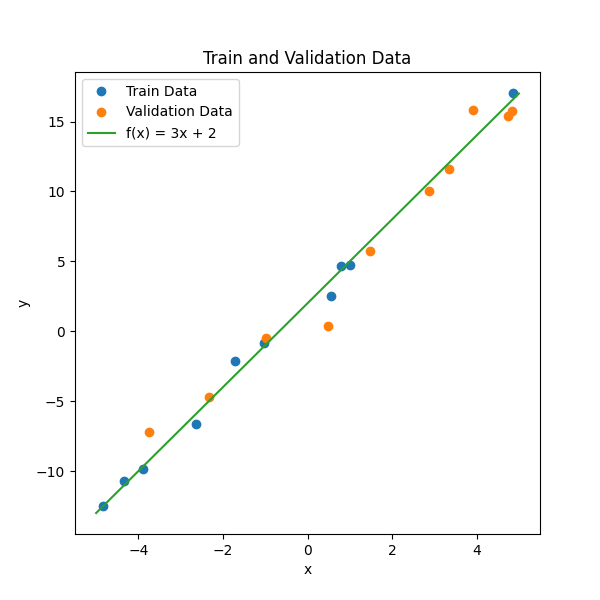
\includegraphics[scale = 0.8]{2a_sample_data.png}

\begin{align}
    RSS = \sum_{n = 1}^{N}(y_{valid, n} - y_{predict, n})^2
\end{align}

where $y_{valid}$ is the $y$ values of the validation data, and $y_{predict}$ are the predicted $y$ values for the validation data using
the ridge regression model trained from our training data, and $N$ is the total number of samples that we are predicting for(In this case, 10).


From (?) we know that $E_{ridge} = ( \A ^T \A + \gamma \I )^{-1} \A ^T \B$. The $A$ matrix for this model is 
\begin{equation*}
    \A =
    \begin{bmatrix}
        1 & x_{train, 1} \\
        1 & x_{train, 2} \\
        1 & x_{train, 3} \\ 
        \vdots & \vdots \\
        1 & x_{train, 10} \\
    \end{bmatrix}
    \B =
    \begin{bmatrix}
        y_{train, 1} \\
        y_{train, 2} \\
        y_{train, 3} \\ 
        \vdots  \\
        y_{train, 10} \\
    \end{bmatrix}
    \x* =
    \begin{bmatrix}
        b \\
        m \\
    \end{bmatrix}
\end{equation*}

We first start with $\gamma = 0$. In that case, the ridge 
estimator reduces to $E_{ridge} = ( \A ^T \A)^{-1} \A ^T \B$ which is just the normal 
equation for standard non penalized least squares. We thus try $\gamma = 0.1$ as well, for our
first real "ridge" regression. -We get the following $RSS$ 

\begin{center}
    \begin{tabular}{||c || c | c ||}
        \hline
        $\gamma$ & 0 & 0.1 \\
        \hline
        $RSS$ & & \\
        \hline
        
    \end{tabular}
\end{center}

We see that we have a lower $RSS$ with $\gamma = 0.1$ rather than $\gamma = 0$. Thus we have already produced a result better than 
non penalized least squares! We have already found a situation where ridge regression is more accurate than non penalized regression.
Now the question is are there any other $\gamma$'s where ridge regression performs better than standard least squares? What is the best $\gamma$?
There is no analytic way to determine the best $\gamma$, so we try a lot of $\gamma$'s and see what happens. First we try 
$\gamma = 0.1, 0.2, 0.3, 0.4, \hdots 10,000$. 


From the graph above we see that the $\gamma$'s with the best $RSS$ are in the interval
$[0,10]$. Thus we now try $\gamma = 0, 0.01, 0.02, 0.03, 0.04, \hdots, 10$

We found minimum $RSS$ to occur at $\gamma = 1$. 

We next move on to using ridge regression for higher degree polynomials. We consider the model 

\begin{equation}
    y = ax^5 + bx^4 + cx^3 + dx^2 + ex + f
\end{equation}

and we will fit $y = x^2$ using the same process as we did for finding the line of best fit. We sample 20 points on the interval $[-5,5)$, take 10 to be our 
training data, and 10 to be our validation data, with Gaussian noise from a standard normal added in. We get the following plot





\end{document}